\chapter{Реализация}

Для работы с L-графами, была написана библиотека на языке Rust. 
Rust -- современный, высокопроизводительный и безопасный язык, библиотеки которого
можно подключить к другим языкам, или использовать механизм WebAssembly для использования
в браузере. Вместе с языком поставляется программа Cargo -- сборщик проектов (build tool) и менеджер
пакетов (package manager). 

В библиотеке реализованы ввод-вывод L-графов в текстовом формате, 
алгоритмы построения ядра L-графа, нормальной формы, и проверка достаточных условий регулярности.

\begin{figure}[h]
    \centering
    \includesvg[scale=0.59, inkscapeformat=png]{images/arch.dot.svg}
    \caption{
        Упрощенная диаграмма классов. Параметр $L$ везде наследует от $Letter$, $N$ -- от $Node$.
        Класс \emph{LGraph<N,L>} содержит в себе и наследует \emph{Graph<N,LGraphLetter<L>{}>}.
        Синим обозначаются интерфейсы, черным -- классы.
        Черные стрелки -- отношение композиции, зеленые -- наследования.
    }
    \label{arch-image}
\end{figure}

\section{Примеры использования библиотеки}

Для начала, требуется установить Rust. Чтобы создать проект Rust с установленной библиотекой,
можно в терминале прописать следующие команды:

\begin{verbatim}
    $ cargo init lgraphs_example
    $ cd lgraphs_example
    $ cargo add --git https://github.com/0Marble/lgraphs.git graphs
    $ cargo build
\end{verbatim}

\begin{figure}
    \centering
    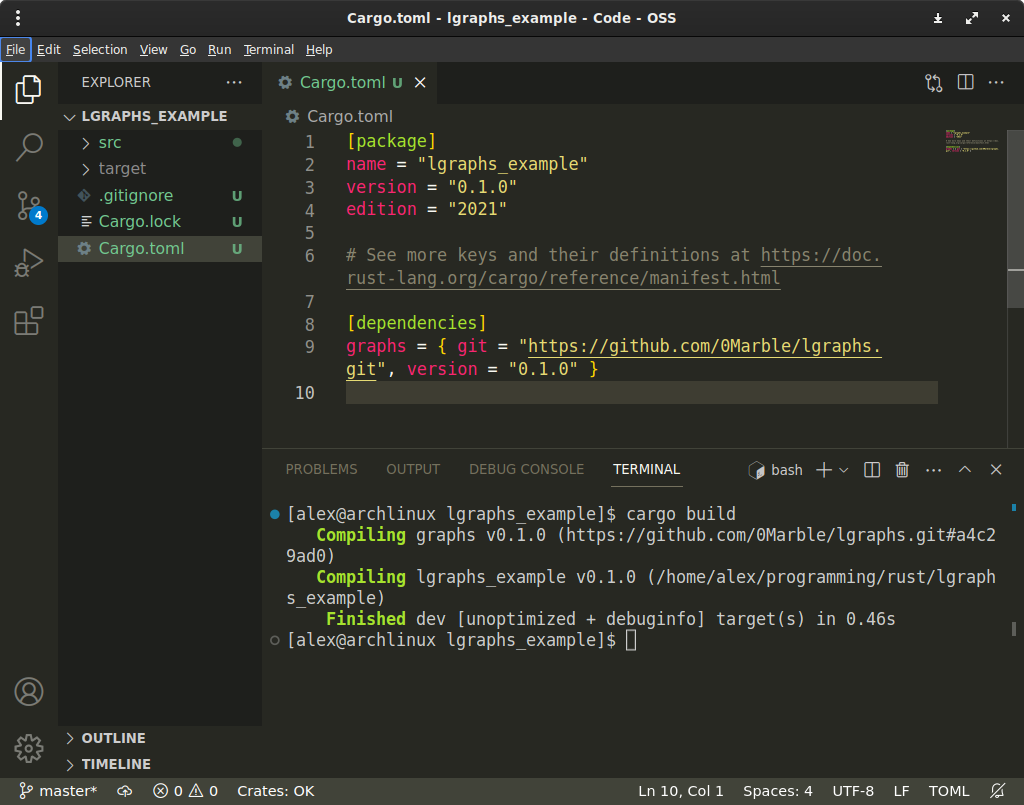
\includegraphics[scale=0.4]{static_images/install_step3.png}
    \caption{Проект с подключенной библиотекой}
    \label{project-setup-image}
\end{figure}

Если все прошло успешно, проект должен выглядеть примерно так, как на рисунке \ref{project-setup-image}.
Теперь, в файле $src/main.rs$ можно писать собственный код.

Разберем несколько примеров программ.

\subsection{Создание и вывод графа}

\inputminted[linenos]{rust}{../lgraphs/examples/helloworld.rs} \label{helloworld-program}

В строках 6-7 создается переменная типа LGraph $g$, который описывается текстом строки-аргумента
метода $from\_str()$. Метод $from\_str()$ может возращать ошибку, поэтому после него ставится $?$, 
что значит ошибка будет автоматически возвращена вызывающей функцией, в данном случае $main()$.

В строках 9-10 мы выводим L-граф в текстом в консоль двумя способами: первый раз выводим по-умолчанию,
в формате, в котором и вводили граф, второй раз используя формат $DOT$ -- известный формат описания графов,
который можно использовать, к примеру, с программой $graphviz$ для рисования графов. 

Для запуска программы, воспользуемся командой
\begin{verbatim}
    $ cargo run
\end{verbatim}
Результат работы показан на рисунке \ref{helloworld-out-image}.

\begin{figure}
    \centering
    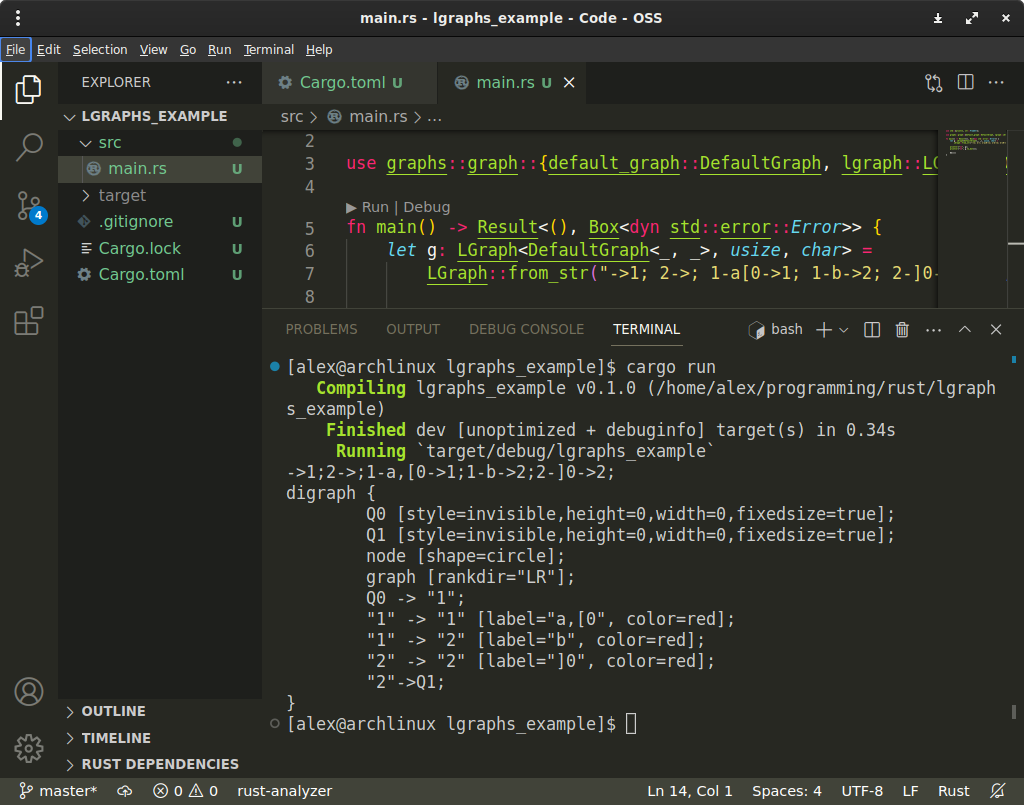
\includegraphics[scale=0.4]{static_images/install_step5.png}
    \caption{Пример запуска программы \ref{helloworld-program}}
    \label{helloworld-out-image}
\end{figure}

\subsection{Вывод ядра L-графа}

\inputminted[linenos]{rust}{../lgraphs/examples/core11.rs} \label{core11-program}

Опять вводим граф $g$ из строки. В строке 9, пробегаем по всем пронумерованным индексом $i$ путям $t$ из ядра $Core(g, 1, 1)$,
полученным вызовом метода $core(1,1)$. Выводим эти строки. Вывод программы в \ref{core11-out-image}.

\begin{figure}
    \centering
    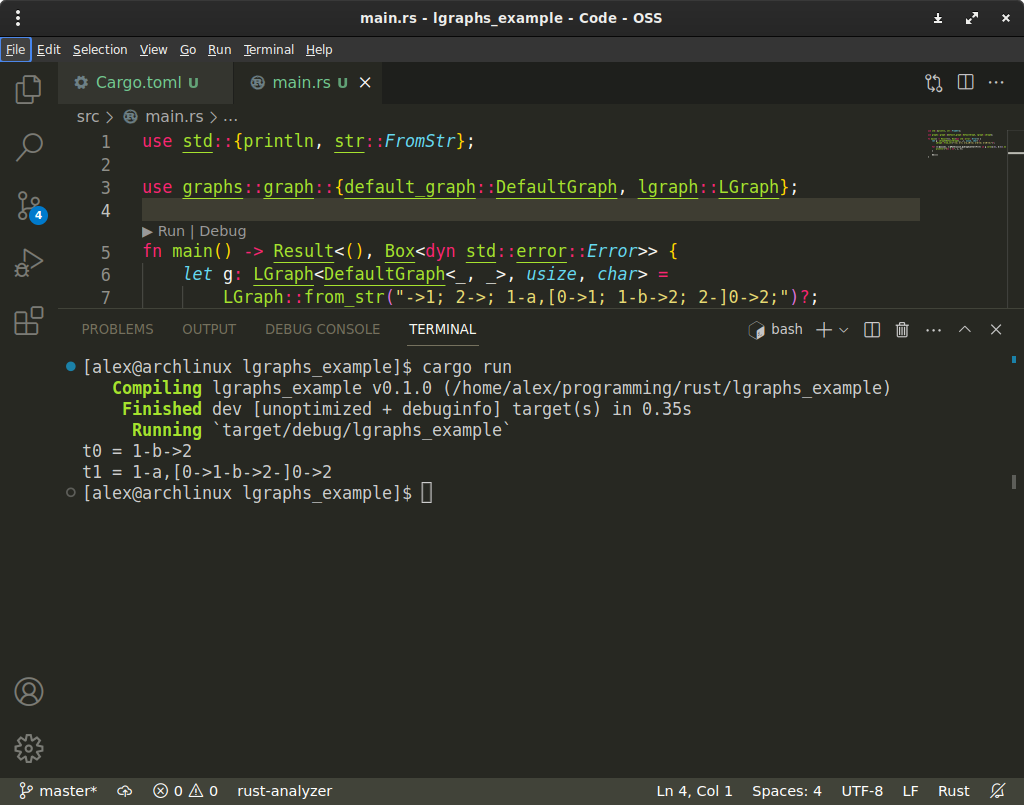
\includegraphics[scale=0.4]{static_images/install_step6.png}
    \caption{Пример запуска программы \ref{core11-program}}
    \label{core11-out-image}
\end{figure}

\subsection{Построение нормальой формы}
\inputminted[linenos]{rust}{../lgraphs/examples/normal.rs} \label{normal-program}

В этой программе следует отметить, что метод $normal\_form()$ требует параметр-тип графа, который является основой
L-графа, поэтому приходится писать \emph{normal\_form::<DefaultGraph<\_, \_> >()}.

В этот раз рассмотрим пример интеграции с языком описания графов $DOT$, и сохраним результат как рисунок.
Для этого требуется установить $graphviz$, после чего можно воспользоваться следующей командой:
\begin{verbatim}
    $ cargo run --example normal | dot -Tpng > mygraph.png
\end{verbatim}

Вывод нашей программы передастся команде $dot$, которая сгенерирует изображение $mygraph$ такого вида,
как на \ref{normal-out-image}.

\begin{figure}[h]
    \centering
    \includesvg[scale=0.4]{static_images/mygraph.svg}
    \caption{Пример запуска программы \ref{normal-program}}
    \label{normal-out-image}
\end{figure}


\pagebreak